\chapter{Influence of loss of control}
\label{chap:loc}

\lettrine{I}{t} is widely believed that \ac{BCI} performance fluctuates over
time due to non-stationary feature distributions \cite{mueller2008mlr,
blankertz2007ics, bunau2009ssa, vidal1977rtd, shenoy2006tac, krauledat2008tzt,
sun2006afe, wolpaw2002bci, jatzev2008ecn}. These non-stationary feature
distributions violate the basic assumption made by the classification models
that the evaluation data (i.e. the online session) is distributed identically
to the data the model was trained on. This problem is known as \emph{covariate shift}, and leads to decreases in the classification performance.
%
Among the hypothesised causes for these non-stationary feature distributions
are changes in the mental state (e.g. fatigue, workload, \ac{LOC}) and
artifacts \cite{blankertz2007ics, jatzev2008ecn}.
\todo{DH: Is LOC een bestaand concept -> kun je meer over zeggen}
%
Although it seems plausible that mental state changes that are detectable in
the \ac{EEG} can interfere with \ac{BCI} operation, there is not much
experimental evidence for this effect. 

In this Chapter, we therefore describe an experiment\footnote{ The work
described in chapter was accepted for publication in the journal IEEE
Transactions of Neural Systems and Rehabilitation Engineering
\cite{reuderink2011ilc}.} we performed to investigate the influence of a
feeling of \ac{LOC} on the detectability of movements with the left and right
index finger through the \ac{EEG}. 
%
Changes in the \ac{EEG} related to users experiencing a state of \ac{LOC} might
lead to a decrease in \ac{BCI} performance due to the aforementioned covariate
shift. In turn, the user state is again influenced by the decreased performance
of the \ac{BCI}; for example, the non-working \ac{BCI} could cause increased
frustration, anger and reduced alertness. This interaction between the user
state and the \ac{BCI} performance might result in a positive feedback loop,
leading to a \ac{BCI} that spins out of control.
%
Given the huge drawbacks of a \ac{BCI} that can stop working depending on the
mental state of a user, understanding the influence of changes in the mental
state on the \ac{BCI} is of great importance to develop reliable \acp{BCI}.

In the following sections we will describe previous work on the relation between
mental states and \ac{BCI} performance, the methods we used, our results, and a
discussion of our experiment, followed by conclusions and directions for future
research.

\section{Previous work}
The influence of frustration associated with \ac{LOC} on a
\ac{BCI} is of great interest since it might cause the previously described
feedback loop. This influence  was previously investigated in
\cite{jatzev2008ecn, zander2009usi}. In this study, users were instructed to
use real movement with their left or right hand to rotate respectively L or
R-shaped objects to a target position in order to study the effect of \acl{LOC}
on the \ac{BCI} performance.
%
The color of the letter indicated the angle of rotation, and the user could
press a key to rotate the object in the direction indicated by the shape of the
object every second.
%
After performing a calibration block with cued left/right hand movement and two
practise blocks with this so-called RLR paradigm, a \ac{LOC} was simulated in
the third block by occasionally using a wrong angle of rotation in the
application. Both an \ac{ERD} and an \ac{ERP} based classifier were trained on
the first block, and applied to the other blocks in an off-line analysis.  A
significant difference between the training block and the \ac{LOC} block was
found for the distribution of \ac{ERD} based features, but for \ac{ERP}
features no such difference was found. This seems to indicate that there is
variability in \ac{ERD} features related to \acl{LOC}. 

However, the study described in \cite{jatzev2008ecn, zander2009usi} is lacking
on a few aspects. Most notable is the limitation that changes in \ac{BCI}
performance due to the induction of \ac{LOC}, the progression of time,
differences in stimulation and user behaviour cannot be distinguished.
%
We were interested in the influence of \ac{LOC} on the \ac{BCI} performance
independent of these other factors. Therefore we used 1) an interleaved block
design to control for effects that manifest spontaneously over time, such as
increasing fatigue, changing temperature, drying gel on the electrodes etc., 2)
we used the same environment for training and evaluating the \ac{BCI}
classifiers to minimize environmental differences not related to \ac{LOC}, 3)
we used self-reported emotional ratings to validate the effect of \acl{LOC} on
the mental state and 4) we tested and corrected for confounding behavioural
changes, such as changes in the force, speed or order of the finger movements,
and eye movements. 

\section{Methods}
During the initiation of imaginary movement, an \ac{ERD} in the $\mu$-band is
often observed in the motor cortices. For \acp{BCI} based on \ac{ERD}, the
spatially filtered \ac{EEG} is used to compute band-power related features
which are then classified with a linear classifier. 

\begin{sloppypar}
Unrelated changes in the \ac{EEG} signal that manifest over time pose a problem
for this classification scheme, because the power, and not the change in power
is used to classify the individual trials. To counter this problem, a pre-trial
baseline is often used in neuroscientific experiments; for
example, the trial power spectrum is often divided by the power spectrum
obtained from a pre-trial baseline to study the \ac{ERD}. Surprisingly,
baselining is rarely used for \acp{BCI}, one exception being
\cite{kronegg2007ebs} where it did indeed result in a performance improvement.
%
In this chapter we propose a new feature domain for \ac{ERD} classification
that uses a multi-variate pre-trial baseline to reduce the covariance between
the \ac{EEG} channels. Before we describe our baselining approach in more
detail, we will re-introduce the \ac{CSP} pipeline that serves as a control in
this work.
\end{sloppypar}

\subsection{CSP classification}\label{sec:CSP}
The \ac{CSP} algorithm  \cite{koles1991qet, ramoser2000osf} was designed to find
a set of $m$ spatial filters that have a maximally different mean variance
(band power) for two classes:
\begin{align}
  \Sigma_{WX} &= I \label{eq:csp_white}\\
  \Sigma_{WX_+} &= D \label{eq:csp_rot},
\end{align}
where $\Sigma_{WX}$ is the channel covariance of the band-pass filtered
\ac{EEG} signal $X$ multiplied by the spatial filter matrix $W$, $X_+$ is the
\ac{EEG} signal generated during one specific task, I is the identity matrix and
D is a diagonal matrix. The \ac{CSP} transform can be decomposed into an
unsupervised whitening transform to satisfy \eqref{eq:csp_white}, and a
class-specific (supervised) linear transformation to satisfy
\eqref{eq:csp_rot}. Usually the $m=6$ filters corresponding to the
$\frac{m}{2}$ smallest and largest eigenvalues in $D$ are used for
classification, as extreme eigenvalues represent projections with the greatest
mean difference in variance.

After projecting a trial to this $m \times n$ space, the logarithm of the
variance of these $m$ projections is typically used as a feature to
automatically train a linear classifier. 
The combination of the feature extraction and a trained classifier results in the follow classification function:
%
\begin{align} \label{eq:csp_lin}
  f(X(i), \vec{w}, W) 
  &= \sum_m w_m \log\left(
    \left(\Sigma_{WX(i)}\right)_{m,m}
    \right) + w_0
\end{align}
with bias $w_0$, feature weights $\vec{w}$, the $m$ spatial filters $W$, and
trial $i$'s band-pass filtered signals $X(i)$. 
%
The variance of the projections is expressed with the diagonal of the
covariance matrix $\diag(\Sigma)$.
%
Traditionally, the logarithm is used to convert the
band-power features to an approximately normal distribution as assumed by
\ac{LDA} classifiers, but the logarithm is not strictly necessary for classification.

\subsection{Direct covariance classification}
\begin{sloppypar}
If we reformulate \eqref{eq:csp_lin} to work in the channel
covariance ($\Sigma_{X(i)}$) space and drop the logarithm:
\begin{align}
  f(\Sigma_{X(i)}, \vec{w}, W) 
  &= \sum_m w_m \left(W\Sigma_{X(i)}W^T\right)_{m,m} + w_0,
\end{align}
%
we can see that $f(\Sigma_{X(i)})$ is just a linear transformation of the
vectorized (flattened) trial covariance matrix denoted by $\vect
\left(\Sigma_{X(i)}\right)$:
%
\begin{align}
  f(\Sigma_{X(i)}, \vec{w}, W) 
  &= \sum_m \vec{w}_m \left(W_{m,\cdot}\Sigma_{X(i)}(W_{m,\cdot})^T\right) + w_0
\\
  &= \sum \left(W^T \diag\left(\vec{w}\right) W\right) \circ \Sigma_{X(i)} + w_0
  \label{eq:filter_fac}
\\
  &= \vec{u}^T \vect\left(\Sigma_{X(i)}\right) + w_0,
  \label{eq:implicit_sf}
\end{align}
where $\circ$ is the Hadamard (element wise) product, $W_{m,\cdot}$ is the m-th
row of $W$, and $\diag\left(\vec{w}\right)$ is a diagonal matrix containing the
values of $\vec{w}$ on its diagonal.
%
The combination of the spatial filters and the band-power feature weights
\begin{align}
  \vec{u} = \vect \left(W^T\diag\left(\vec{w}\right)W\right)
\end{align}
can thus be modeled directly with a regularized linear classifier
\cite{farquhar2009lfs}. This simplification enables the classifier to learn
spatial filters simultaneously with the projection's variance weighting in a
single, supervised learning step. 
\end{sloppypar}

For direct covariance classification, we have chosen to explicitly decorrelate
the channels with a symmetric whitening transform $P$ that is estimated on the
training trials to satisfy \eqref{eq:csp_white}:
\begin{equation}
  P = \Sigma_X^{-\frac{1}{2}} = U \Lambda^{-\frac{1}{2}} U^T 
    \quad \text{with} \quad U \Lambda U^T = \Sigma_X,
    \label{eq:white}
\end{equation}
and only learn the rotational spatial filters and their associated weights
implicitly as in \eqref{eq:implicit_sf}  with a linear \ac{SVM}. Without this
whitening transform, the \ac{SVM}'s $\ell_2$ regulariser strongly biasses the
classifier to focus on high-powered sources that are probably not
originating form the brain.

In summary, we used the covariance of whitened trials as features to directly
train a linear classifier that is, except for the log transform, almost
equivalent to the commonly used \ac{CSP} pipeline.

\subsection{Covariance classification with a second order-baseline}
Likewise, the proposed \acf{SOB} method learns the spatial filters implicitly,
but instead of the static whitening transform \eqref{eq:white} a pre-trial
baseline is used to \emph{adaptively} normalize ongoing second order covariance
statistics.

We estimated a whitening transform $P(i)$ for each trial $i$ based on past
pre-trial baselines, and applied this transform to the data of the trial itself.
Without a change in brain activity, the covariance during normalized trial
$P(i)X(i)$ would approximate the identity matrix, even during (slow) sensor
covariance changes. But when the coupling between or the power in certain
brain regions changes, a perturbation appears in the sensor covariance during
the normalized trial. This perturbation can be used for classification.
%
The specific whitening transform \eqref{eq:white} has the crucial property that
it removes correlations, but at the same time minimizes the distorting to
preserve the relation between projections and locations on the scalp. This
preserves the task-relevant topography, which is needed to have consistent
features over time and over subjects.
%
A similar normalization procedure was outlined in \cite{tomioka2006asf} to
adapt the session covariance matrix in order to reduce the influence of
non-stationarities. The main differences between our method and
\cite{tomioka2006asf} is that in our method each trial is normalized
differently based on the pre-trial baseline, and that this baseline period is
used to estimate the resting state covariance instead of the global session
covariance.

\begin{sloppypar}
Estimating the symmetrical whitening transform from the pre-trial baseline
covariance $\Sigma_{B(i)}$ for trial $i$ is difficult, since there is a large
number of parameters to estimate from a few independent samples for the $s$
sensors. To improve the robustness, we used the regularized Ledoit-Wolf
covariance estimator \cite{ledoit2004wce}, and used an \ac{EWMA} to combine the
baseline covariance of past trials into a covariance estimate $\Sigma_B(i)$
for the baseline of trial $i$:
%
\begin{equation} 
  \hat\Sigma_{B(i)} = \alpha S^*_{B(i)} + (1 - \alpha) \hat\Sigma_{B(i-1)}, 
\end{equation} 
%
where $S^*_{B(i)}$ is the Ledoit-Wolf covariance estimate of the baseline before
trial $i$, and $\alpha$ is known as the forgetting factor that determines the
rate of adaptation. With 
\begin{align}
  \alpha = 1-\sqrt[n]{\tfrac{1}{2}}
\end{align}
%
the forgetting factor $\alpha$ is then associated with a decay that halves in
$n$ trials.
\end{sloppypar}

Specifically, we calculate a whitening transform $P(i)$ for each of
the trials $X(i)$ based on $\hat\Sigma_{B(i)}$, and apply this $P(i)$ to the Ledoit-Wolf covariance estimate of
the current trial $S^*_{X(i)}$:
%
\begin{equation}
\tilde{X(i)} = P(i) S^*_{X(i)} P(i)^T \quad \text{with} \quad 
  P(i) = \Sigma_{B(i)}^{-\frac{1}{2}}.
\end{equation}
The new features $\vect \left(\tilde{X(i)}\right)$ are more robust against time
and subject related variations, but are still sensitive to task-related (co)variance changes.

\subsection{Dataset}
To evaluate the performance of the invariant features we used the movement
imagery dataset\footnote{\url{http://www.physionet.org/pn4/eegmmidb/}} from the
experiment described in \cite{schalk2004bgp} contributed to Physiobank
\cite{goldberger2000ppp}. This dataset contains sessions of 109 different
subjects with trials for actual and imagined movement \cite{schalk2011pc}.
The \ac{EEG} was recorded with 64 electrodes positioned spread over the scalp according to the international 10-10 system, sampled at 160~Hz.

\begin{sloppypar}
We have chosen to use the blocks where the subjects had to imagine either
movement of both feet or movement with both hands, as a preliminary experiment
indicated that \ac{BCI} classification performance above chance level can be
obtained with small training sets. There are about 22 trial per class for each
subject.
\end{sloppypar}

\subsection{Preprocessing}
To preprocess the data, we applied a 6th-order Butterworth notch filter at
60~Hz, applied a 6th-order Butterworth filter between 8--30~Hz and extracted
trials for movement imagery of both hands or of both feet in the interval from
$[-2, 4]$~s after the stimulus. 
%
All evaluated methods used the same interval $[0.5, 4]$~s after the stimulus
presentation for classification. For the \ac{SOB} method, the interval $[-2,
0]$~s was used to estimate the pre-trial baseline. The same preprocessing was
used for all \ac{BCI} classifiers.

\subsection{Evaluation}
\begin{sloppypar}
We used two \ac{CSP}-based pipelines and a \ac{logBP} based pipeline as a
comparison method in both an \ac{SD} and an \ac{SI} \ac{BCI} classification
scheme. One \ac{CSP} pipeline was based on \ac{CSP} projected log band-power
features classified with an \ac{LDA}, the other \ac{CSP} classifiers used
band-power features without the log transform, classified with a linear
soft-margin \ac{SVM} \cite{cortes1995svn}. The \ac{logBP} classifiers simply
used the variance of each band-pass filtered channel as a feature for a linear
\ac{SVM}. The whitened covariance features and \ac{SOB} normalized covariance
features were also classified with a linear \ac{SVM}. The \ac{SVM}'s
$c$-parameter was always estimated using a sequential (chronological) 5-fold
cross-validation procedure with a logarithmic step size for the $c$-values, on
the training set.
\end{sloppypar}

To evaluate these classifiers in an \ac{SD} context, the first half of the
session was used for training, and the second half was used for evaluation.
This simulates a calibration and application session, respectively.
Chronological separation of training and test set is needed since random splits
lead to overly optimistic performance estimates. As the dataset also
contains blocks with other mental tasks, we have only about 22 trials in total
for training and 22 trials for evaluation per subject.

The performance of \ac{SI} application was assessed by training an \ac{SI}
classifier on the first 50 users, and then applying the classifier to the test
set formed from the remaining 51 subjects (we removed 8 subjects from the test
pool because they had fewer trials). The final \ac{SI} performance was
calculated on the second half of the predictions for these 51 test subjects to
allow for a paired comparison with the \ac{SD} classifiers.

\section{Results}
\subsection{Subjects}
Twelve healthy users (age $27 \pm 3.9$) participated in the experiment.  All
participants had normal, or corrected to normal vision, and reported not to use
medication. Only three of our subjects were female, and all subjects were
right-handed. Most participants had some video game experience, and four
subjects had previous experience with \acp{BCI}.

\subsection{Self assessments}
To verify the induction of changes in the mental state, we analysed the self
reported emotional ratings of the \ac{SAM}. Most subjects rated the \ac{LOC}
condition more negatively than the normal condition, over subjects this
difference was significant ($T$=3, $p$\textless 0.01). While we expected to
find a trend towards more arousal in the \ac{LOC} condition, there was no
significant difference ($T$=23, $p$=0.26). The dominance dimension, which
measures the amount of dominance, or control they have on their environment,
indicate that people seemed to be significantly ($T$=3.5, $p$\textless 0.01)
more in control in the normal condition.


\begin{figure}
  \center
  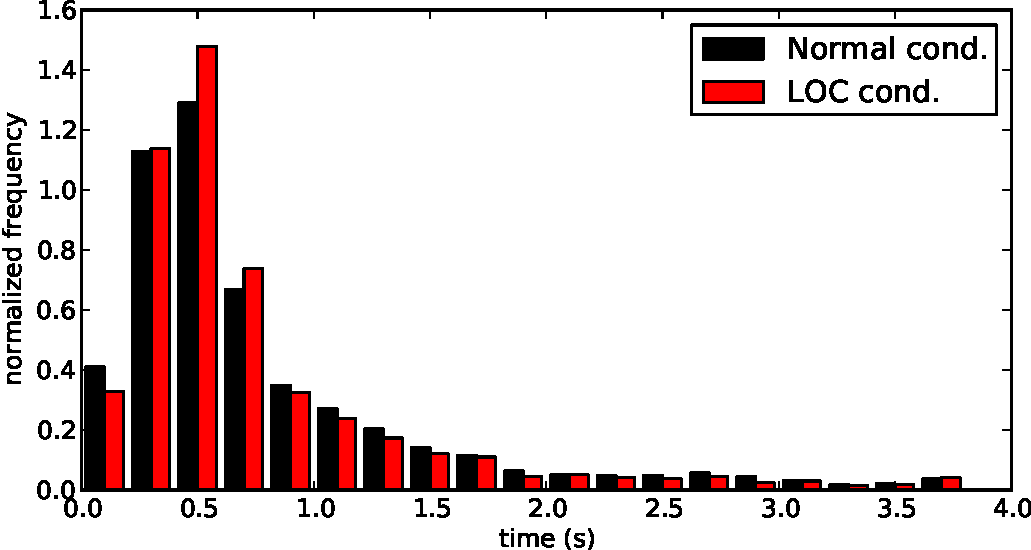
\includegraphics[width=3.5in]{key_duration.pdf}
  \caption{The histogram for the time between key presses during game play for
  all subjects. The intervals for the normal condition are displayed in black,
  the \protect\ac{LOC} condition is displayed in red (gray). The histogram is
  dominated by short $\Delta t$'s between key presses. The histogram of the
  \protect\ac{LOC} condition seems to be slightly more pinched around half a
  second.}
  \label{fig:key_duration}
\end{figure}

\begin{figure}
  \center
  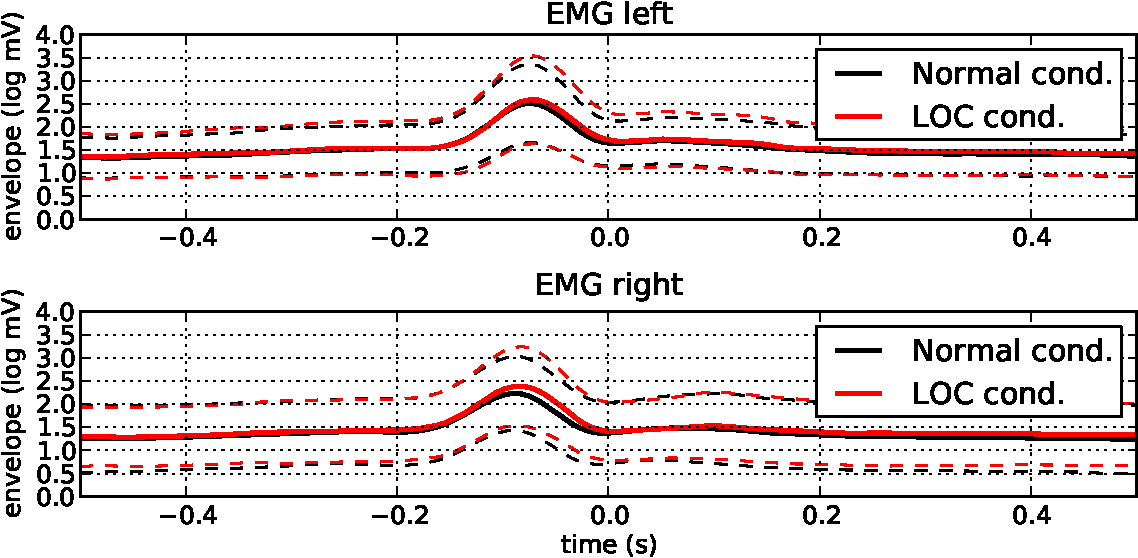
\includegraphics[width=3.5in]{emg_cond.pdf}
  \caption{The mean log \protect\ac{EMG} power and its standard deviation
  (dashed lines) is displayed for both the normal and \protect\ac{LOC}
  condition, time-locked to the key press at $t=0$. The top plot shows the EMG
  power of the left bipolar channel for left index-finger presses, the bottom
  plot show the EMG power for right hand movement measured with the right
  bipolar channel.}
  \label{fig:emg_cond}
\end{figure}

\begin{table}
  \caption{Statistics of confounding variables. The repetitiveness (second
  column) and log-\protect\ac{EMG} power (last column) differ significantly
  between the conditions. The \protect\ac{EMG} power was quantified as the
  maximum power in the interval [-0.2,~0]~s. The start and end of the arrow
  signify the mean value in the normal and \protect{LOC} condition
  respectively.} 
  \center \footnotesize
  \begin{tabular}{c c c c c}
\toprule
 & log $\Delta t$ & $p(y_t=y_{t-1})$ & log pow. EMG L & log pow. EMG R\\
\midrule
S0 & -0.48 $\rightarrow$ -0.36 &  0.51 $\rightarrow$  0.59 &  1.31 $\rightarrow$  1.21 &  1.08 $\rightarrow$  1.15\\
S1 & -0.51 $\rightarrow$ -0.53 &  0.54 $\rightarrow$  0.59 &  2.70 $\rightarrow$  2.60 &  2.04 $\rightarrow$  2.17\\
S2 & -0.54 $\rightarrow$ -0.59 &  0.50 $\rightarrow$  0.52 &  2.65 $\rightarrow$  2.58 &  2.51 $\rightarrow$  2.46\\
S3 & -0.47 $\rightarrow$ -0.61 &  0.56 $\rightarrow$  0.54 &  1.99 $\rightarrow$  1.88 &  2.15 $\rightarrow$  2.31\\
S4 & -0.46 $\rightarrow$ -0.55 &  0.53 $\rightarrow$  0.58 &  3.14 $\rightarrow$  3.35 &  1.76 $\rightarrow$  1.86\\
S5 & -0.46 $\rightarrow$ -0.44 &  0.56 $\rightarrow$  0.60 &  2.70 $\rightarrow$  2.56 &  4.06 $\rightarrow$  3.91\\
S6 & -0.46 $\rightarrow$ -0.48 &  0.55 $\rightarrow$  0.55 &  2.11 $\rightarrow$  2.55 &  2.14 $\rightarrow$  2.47\\
S7 & -0.40 $\rightarrow$ -0.55 &  0.58 $\rightarrow$  0.56 &  1.70 $\rightarrow$  1.71 &  2.13 $\rightarrow$  2.14\\
S8 & -0.37 $\rightarrow$ -0.44 &  0.47 $\rightarrow$  0.56 &  2.89 $\rightarrow$  2.95 &  2.94 $\rightarrow$  3.02\\
S9 & -0.58 $\rightarrow$ -0.55 &  0.45 $\rightarrow$  0.54 &  3.02 $\rightarrow$  3.08 &  2.01 $\rightarrow$  2.06\\
S10 & -0.58 $\rightarrow$ -0.44 &  0.47 $\rightarrow$  0.53 &  2.43 $\rightarrow$  2.42 &  2.52 $\rightarrow$  2.55\\
S11 & -0.45 $\rightarrow$ -0.42 &  0.52 $\rightarrow$  0.58 &  3.01 $\rightarrow$  2.86 &  2.97 $\rightarrow$  3.13\\
\midrule
mean & -0.48 $\rightarrow$ -0.50 &  0.52 $\rightarrow$  0.56 &  2.47 $\rightarrow$  2.48 &  2.36 $\rightarrow$  2.44\\
Wilc. & T=32, p=0.583 & \textbf{T=6, p=0.010} & T=31, p=0.530 & \textbf{T=12, p=0.034}\\
\bottomrule
\end{tabular}

  \label{tab:confounds} 
\end{table}

\subsection{Confounding behavioural differences} \label{sec:behav} 
In this section we describe the analysis of the characteristics of the user's
behaviour, as it might have had a confounding influence on the \ac{BCI}
performance. 
%
Both differences in the \ac{ITI}, and the pattern of consecutive keystrokes
can indicate a confounding behavioural change. The per-subject statistics for
these confounding factors are presented in Table~\ref{tab:confounds}. For the
log \ac{ITI}, we see an insignificant tendency to shorter intervals between key
presses in the \ac{LOC} condition. The probability that a key press was made
with the same hand is significantly higher in the \ac{LOC} condition. This may have been caused by increased repetition, by increased imbalance of the class ratios,
or a combination thereof. Nevertheless, it indicates a significant behavioural
change.

The temporal development of the \ac{EMG} signal is displayed in
Fig.~\ref{fig:emg_cond}. An increase in the \ac{EMG} power is visible just
before the stroke is registered, and a much weaker increase is visible when the
key is released. Most of the activity is registered in the interval [-0.2, 0]~s
relative to the registration of the key press. We used the maximum \ac{EMG}
power in this interval to estimate the force used to press a key (see
Table~\ref{tab:confounds}). Movements with the right index finger produce
significantly more \ac{EMG} power in the \ac{LOC} condition.

\begin{figure}
  \center
  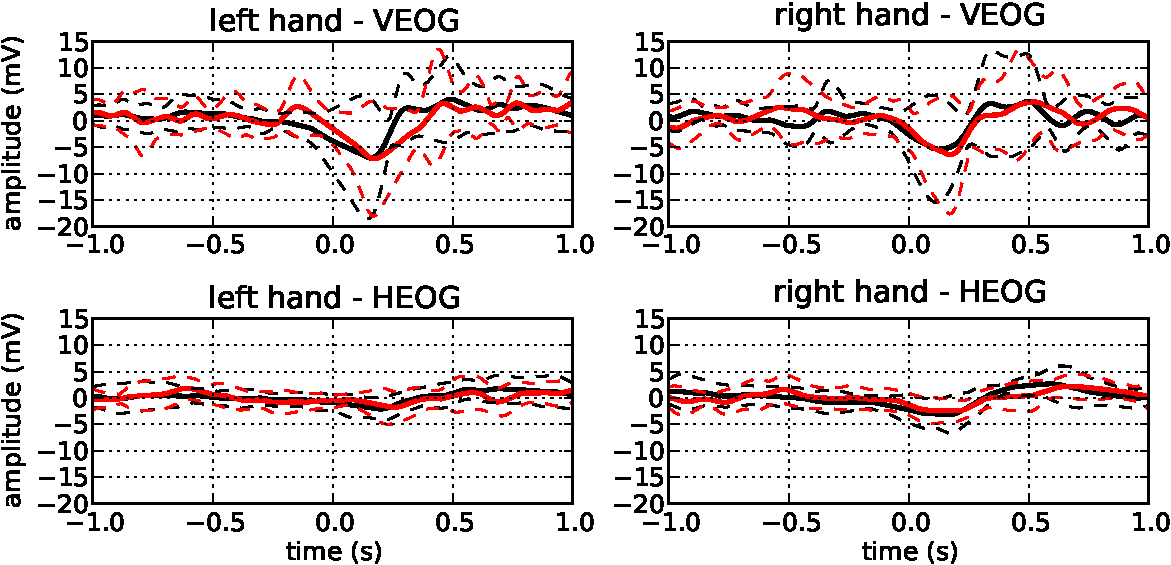
\includegraphics[width=\textwidth]{eog_cond.pdf}
  \caption{The vertical eye movement (first row) show downward eye-gaze just
  after a keystroke at $t=0$. The horizontal bipolar \protect\ac{EOG} channel
  is rather uneventful, only for right hand movement (last column) does there
  appear to be a delayed reaction to the key press, first negative (looking
  left) then positive (looking right). The dashed lines indicate the standard
  deviation.  There is no significant difference (16 point Bonferroni corrected
  Wilcoxon signed-rank test over subjects) between the normal (black) and
  \protect\ac{LOC} condition (red).}
  \label{fig:eog_cond}
\end{figure}

Although we removed (most) of the influence of the \ac{EOG} signal from the
\ac{EEG}, it is interesting to look at the user's gaze and blink behaviour
during a key press (Fig.~\ref{fig:eog_cond}). We can see that users tend to
look at their hands 200~ms after a key press, which is most visible in the
vertical \ac{EOG}, and at 300~ms, the variability of the vertical \ac{EOG}
signal seems to increase. This might be caused by eye-blinks, or an adjustment
to the new movement direction of the avatar in the game. 

In summary, our behaviour analysis has shown that the normal and
\ac{LOC}-con\-di\-tions are very similar in the timing, the predictability of
the key\-strokes, the amount of force used to press the keys, and in eye
movements. However, there was a small but significant increase in repetition of
the same movement, and a small significant increase in the force used with the
right hand. After balancing the confounding variables and their interactions
per subject, on average 25\% of the original trials were removed.

\subsection{Impact of loss of control on the BCI}
To investigate the influence of \ac{LOC} on the \ac{BCI} performance, we
trained the \ac{ERD} based and the \ac{ERP}-based classifier on blocks from the
normal condition, and compared the performance on unseen normal blocks with the
performance on blocks from the \ac{LOC} condition. Please refer to
Section~\ref{sec:dga} for more information on this procedure.

\begin{table*} 
  \caption{The influence of \protect\ac{LOC} on a \protect\ac{CSP} classifier
  is shown below, without correction for confounding factors. The start and end
  of the arrow indicate the median performance for the normal and
  \protect\ac{LOC} condition respectively. The $p$-value of a Mann-Whitney U
  test on the per-block performance is displayed above the arrow. The row
  denoted with ``Wilc.'' signifies the over-subject comparison with the Wilcoxon
  signed rank test. The row denoted by ``Fish.'' presents the results of
  combining one-sided $p$-values for an increase in performance.}
  \center \scriptsize
  \begin{tabular}{c c c c c}
\toprule
 & Accuracy & AUC & MI & ITR\\
\midrule
S0 &  0.679 $\xrightarrow{p=0.35}$  0.736 &  0.759 $\xrightarrow{p=0.35}$  0.843 &  0.110 $\xrightarrow{p=0.35}$  0.193 & 11.680 $\xrightarrow{p=0.48}$ 13.763\\
S1 &  0.599 $\xrightarrow{p=0.48}$  0.618 &  0.616 $\xrightarrow{p=0.64}$  0.652 &  0.021 $\xrightarrow{p=0.64}$  0.041 &  2.601 $\xrightarrow{p=0.64}$  4.525\\
S2 &  0.619 $\xrightarrow{p=0.92}$  0.555 &  0.543 $\xrightarrow{p=0.62}$  0.578 &  0.001 $\xrightarrow{p=0.77}$  0.000 &  0.088 $\xrightarrow{p=0.92}$  0.025\\
S3 &  0.474 $\xrightarrow{p=0.13}$  0.519 & \textbf{ 0.466 $\xrightarrow{p=0.05}$  0.518} &  0.004 $\xrightarrow{p=0.62}$  0.003 &  0.452 $\xrightarrow{p=0.77}$  0.338\\
S4 &  0.519 $\xrightarrow{p=0.92}$  0.507 &  0.549 $\xrightarrow{p=0.92}$  0.526 &  0.002 $\xrightarrow{p=0.77}$  0.003 &  0.224 $\xrightarrow{p=0.77}$  0.351\\
S5 &  0.741 $\xrightarrow{p=0.92}$  0.750 &  0.828 $\xrightarrow{p=0.92}$  0.832 &  0.167 $\xrightarrow{p=0.92}$  0.188 & 15.616 $\xrightarrow{p=0.92}$ 20.297\\
S6 &  0.538 $\xrightarrow{p=0.65}$  0.529 &  0.543 $\xrightarrow{p=0.86}$  0.522 &  0.003 $\xrightarrow{p=0.59}$  0.006 &  0.302 $\xrightarrow{p=0.59}$  0.664\\
S7 &  0.544 $\xrightarrow{p=0.10}$  0.600 &  0.565 $\xrightarrow{p=0.27}$  0.657 &  0.005 $\xrightarrow{p=0.19}$  0.027 &  0.532 $\xrightarrow{p=0.08}$  3.082\\
S8 &  0.542 $\xrightarrow{p=0.34}$  0.581 &  0.556 $\xrightarrow{p=0.34}$  0.589 &  0.004 $\xrightarrow{p=0.48}$  0.010 &  0.366 $\xrightarrow{p=0.48}$  1.035\\
S9 &  0.735 $\xrightarrow{p=0.15}$  0.768 &  0.797 $\xrightarrow{p=0.15}$  0.839 &  0.160 $\xrightarrow{p=0.15}$  0.218 & 18.879 $\xrightarrow{p=0.15}$ 24.494\\
S10 &  0.612 $\xrightarrow{p=0.35}$  0.582 &  0.670 $\xrightarrow{p=0.48}$  0.651 &  0.046 $\xrightarrow{p=0.35}$  0.018 &  5.611 $\xrightarrow{p=0.35}$  2.108\\
S11 &  0.608 $\xrightarrow{p=0.34}$  0.553 &  0.594 $\xrightarrow{p=0.95}$  0.599 &  0.020 $\xrightarrow{p=0.95}$  0.023 &  2.371 $\xrightarrow{p=0.64}$  2.059\\
\midrule
mean & 0.601 $\rightarrow$ 0.608 & 0.624 $\rightarrow$ 0.651 & 0.045 $\rightarrow$ 0.061 & 4.893 $\rightarrow$ 6.062\\
Wilc. & T=31.0, p=0.530 & \textbf{T=12.0, p=0.034} & \textbf{T=14.0, p=0.050} & T=17.0, p=0.084\\
%Fish. 2-way & p=0.469 & p=0.643 & p=0.846 & p=0.793\\
Fish. & p=0.123 & p=0.078 & p=0.259 & p=0.222\\
%Fish. 1-way - & p=0.912 & p=0.986 & p=0.947 & p=0.941\\
\bottomrule
\end{tabular}

  \label{tab:csp}
\end{table*}

\begin{table*} 
  \caption{The influence of \protect\ac{LOC} on a \protect\ac{CSP} classifier
  is shown below, with correction for confounding factors enabled. Please refer
  to Table~\ref{tab:csp} for an explanation. } 
  \center \scriptsize
  \begin{tabular}{c c c c c}
\toprule
 & Accuracy & AUC & MI & ITR\\
\midrule
S0 &  0.678 $\xrightarrow{p=0.64}$  0.667 &  0.718 $\xrightarrow{p=0.35}$  0.785 &  0.094 $\xrightarrow{p=0.82}$  0.056 &  7.370 $\xrightarrow{p=0.95}$  4.896\\
S1 & \textbf{ 0.543 $\xrightarrow{p=0.05}$  0.646} &  0.572 $\xrightarrow{p=0.09}$  0.686 & \textbf{ 0.007 $\xrightarrow{p=0.05}$  0.063} &  0.734 $\xrightarrow{p=0.09}$  6.751\\
S2 &  0.640 $\xrightarrow{p=1.00}$  0.626 &  0.558 $\xrightarrow{p=0.92}$  0.548 &  0.009 $\xrightarrow{p=0.19}$  0.002 &  0.825 $\xrightarrow{p=0.27}$  0.165\\
S3 &  0.541 $\xrightarrow{p=0.62}$  0.553 &  0.483 $\xrightarrow{p=0.62}$  0.514 &  0.007 $\xrightarrow{p=0.77}$  0.005 &  0.482 $\xrightarrow{p=0.62}$  0.450\\
S4 &  0.569 $\xrightarrow{p=0.19}$  0.532 &  0.572 $\xrightarrow{p=0.77}$  0.536 &  0.013 $\xrightarrow{p=0.92}$  0.008 &  1.416 $\xrightarrow{p=0.92}$  0.769\\
S5 &  0.753 $\xrightarrow{p=0.77}$  0.743 &  0.857 $\xrightarrow{p=0.62}$  0.821 &  0.198 $\xrightarrow{p=0.77}$  0.180 & 14.086 $\xrightarrow{p=0.77}$ 15.423\\
S6 &  0.532 $\xrightarrow{p=0.21}$  0.558 & \textbf{ 0.498 $\xrightarrow{p=0.01}$  0.579} &  0.004 $\xrightarrow{p=0.10}$  0.011 &  0.308 $\xrightarrow{p=0.06}$  0.874\\
S7 &  0.549 $\xrightarrow{p=0.37}$  0.577 &  0.613 $\xrightarrow{p=0.92}$  0.623 &  0.010 $\xrightarrow{p=0.49}$  0.015 &  0.964 $\xrightarrow{p=0.37}$  1.534\\
S8 &  0.543 $\xrightarrow{p=0.48}$  0.605 &  0.549 $\xrightarrow{p=0.23}$  0.583 & \textbf{ 0.002 $\xrightarrow{p=0.02}$  0.017} & \textbf{ 0.166 $\xrightarrow{p=0.02}$  1.394}\\
S9 &  0.687 $\xrightarrow{p=0.23}$  0.740 &  0.783 $\xrightarrow{p=0.23}$  0.833 &  0.086 $\xrightarrow{p=0.15}$  0.162 &  8.770 $\xrightarrow{p=0.15}$ 16.045\\
S10 & \textbf{ 0.658 $\xrightarrow{p=0.05}$  0.617} &  0.676 $\xrightarrow{p=0.82}$  0.673 &  0.054 $\xrightarrow{p=0.24}$  0.035 &  4.888 $\xrightarrow{p=0.35}$  3.147\\
S11 &  0.585 $\xrightarrow{p=0.23}$  0.551 & \textbf{ 0.615 $\xrightarrow{p=0.01}$  0.544} &  0.021 $\xrightarrow{p=0.23}$  0.005 &  1.329 $\xrightarrow{p=0.15}$  0.366\\
\midrule
mean & 0.606 $\rightarrow$ 0.618 & 0.625 $\rightarrow$ 0.644 & 0.042 $\rightarrow$ 0.047 & 3.445 $\rightarrow$ 4.318\\
Wilc. & T=31.0, p=0.530 & T=27.0, p=0.347 & T=35.0, p=0.754 & T=35.0, p=0.754\\
%Fish. 2-way & p=0.172 & p=0.077 & p=0.081 & p=0.083\\
Fish. & p=0.237 & \textbf{p=0.050} & p=0.063 & \textbf{p=0.047}\\
%Fish. 1-way - & p=0.443 & p=0.602 & p=0.622 & p=0.707\\
\bottomrule
\end{tabular}

  \label{tab:csp_bal}
\end{table*}

The performance of the \ac{CSP} based features classifier on the normal and
\ac{LOC} blocks without correction for confounds is displayed in
Table~\ref{tab:csp}. The single trial detection accuracy may seem rather low
(60\%), but this is similar to the accuracies obtained in other studies that
use short \acp{ITI}, such as \cite{jatzev2008ecn}. This was also reflected in
the mean \ac{ITR} of 5.5 bits per minute, which is comparable to the \acp{ITR}
obtained by naive users with motor-imagery based \ac{ERD} \acp{BCI}.
%
Despite this low recognition rate, the \ac{ERD} \acp{BCI} performance did
significantly \emph{increase} in the \ac{LOC} condition for the \ac{AUC} and
\ac{MI} measures.

When correction for confounding factors was performed, the results were
different (Table~\ref{tab:csp_bal}); the over-subject differences disappeared,
but there were more significant within-subject differences in sometimes opposing
directions. Combined with Fisher's method, the one-sided $p$-values for a
within-subject increase in performance was significant for both \ac{AUC} and
\ac{ITR}. This indicates at least one individual increase in performance was
significant at the $\alpha=0.05$ level.

\begin{sidewaysfigure}
  \centering
  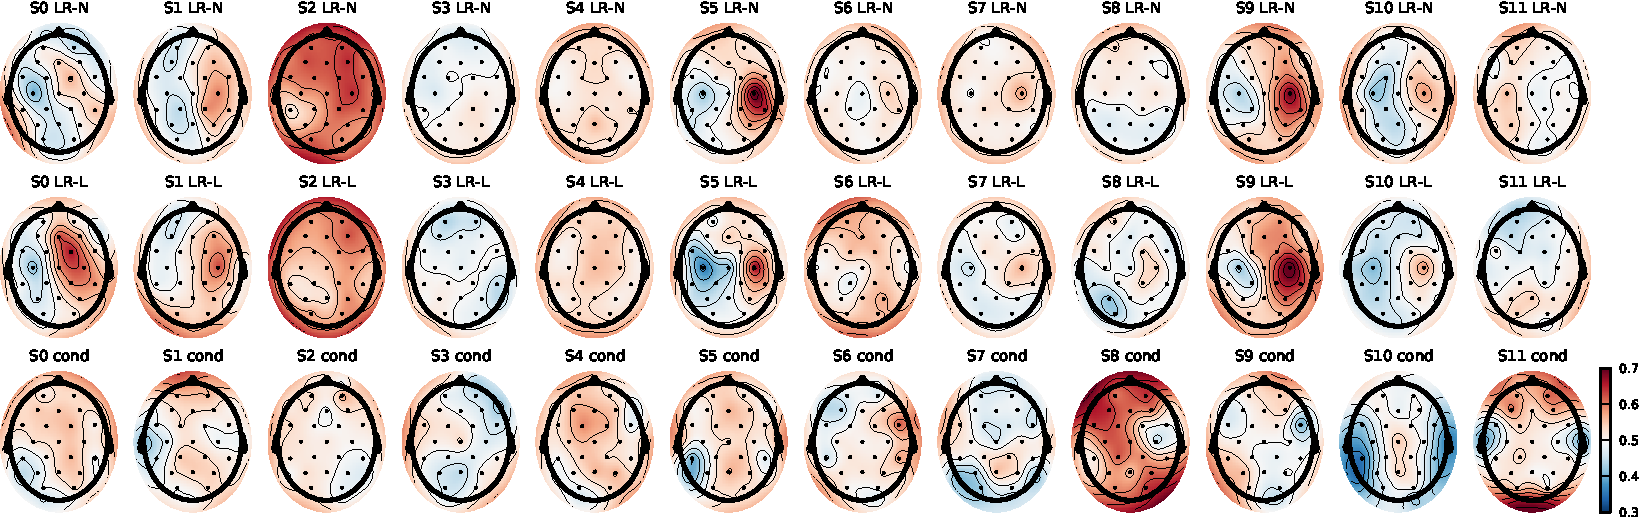
\includegraphics[width=\textwidth]{figs/bp_nlc.pdf}
  \caption{
  These scalp plots display the difference between left and right hand movement
  in the normal (first row) and \protect\ac{LOC} condition (second row), and
  the difference between the normal and \protect\ac{LOC} in the last row. 
  %
  The color encodes the \protect\ac{AUC}-\protect\ac{ROC} ranking performance
  of the 8--30~Hz band power at the specified location; red indicates a
  positive rank correlation with the target class (right hand for the first two
  rows, or \protect\ac{LOC} in the last), blue a negative correlation. The
  conditions were corrected for confounding factors with frequency matching.
  %
  Most subjects display a more pronounced spatial activation in
  the \protect\ac{LOC} condition.}
  \label{fig:ERD_diff} 
\end{sidewaysfigure}

\begin{sloppypar}
The spatial distribution of the movement related \ac{ERD} is shown in
Fig.~\ref{fig:ERD_diff}. Subjects S0, S1, S5,  S9 and S10 do display the
prototypical \ac{ERD} on the motor cortices. Remarkably, these activations are
more pronounced in the \ac{LOC} condition (second row), which supports the
observed increase in performance. 
%
Note that the \ac{CSP} classification is based on covariance of the \ac{EEG}
channels, while in this figure only the variance is shown. 
\end{sloppypar}


\begin{table*}
  \caption{The influence of \protect\ac{LOC} on a \protect\ac{ERP} classifier
  is shown below, without correction for confounding factors. Please refer to
  Table~\ref{tab:csp} for an explanation.}
  \center \scriptsize
  \begin{tabular}{c c c c c}
\toprule
 & Accuracy & AUC & MI & ITR\\
\midrule
S0 &  0.765 $\xrightarrow{p=0.73}$  0.747 &  0.824 $\xrightarrow{p=0.95}$  0.812 &  0.223 $\xrightarrow{p=0.64}$  0.179 & 24.349 $\xrightarrow{p=0.48}$ 17.575\\
S1 &  0.802 $\xrightarrow{p=0.34}$  0.758 &  0.866 $\xrightarrow{p=0.64}$  0.823 &  0.282 $\xrightarrow{p=0.23}$  0.195 & 32.838 $\xrightarrow{p=0.34}$ 22.092\\
S2 &  0.726 $\xrightarrow{p=0.27}$  0.750 &  0.790 $\xrightarrow{p=0.49}$  0.809 &  0.142 $\xrightarrow{p=0.62}$  0.154 & 16.269 $\xrightarrow{p=0.37}$ 18.677\\
S3 &  0.711 $\xrightarrow{p=0.77}$  0.724 &  0.779 $\xrightarrow{p=0.62}$  0.788 &  0.133 $\xrightarrow{p=0.77}$  0.139 & 11.719 $\xrightarrow{p=0.77}$ 16.195\\
S4 &  0.692 $\xrightarrow{p=0.92}$  0.714 &  0.767 $\xrightarrow{p=0.37}$  0.803 &  0.096 $\xrightarrow{p=0.92}$  0.110 & 11.672 $\xrightarrow{p=0.77}$ 11.882\\
S5 &  0.720 $\xrightarrow{p=0.77}$  0.715 &  0.800 $\xrightarrow{p=0.92}$  0.790 &  0.142 $\xrightarrow{p=0.92}$  0.136 & 14.584 $\xrightarrow{p=0.62}$ 15.041\\
S6 &  0.703 $\xrightarrow{p=0.15}$  0.726 &  0.766 $\xrightarrow{p=0.15}$  0.789 &  0.116 $\xrightarrow{p=0.10}$  0.155 & 13.460 $\xrightarrow{p=0.10}$ 16.812\\
S7 &  0.772 $\xrightarrow{p=0.77}$  0.778 &  0.833 $\xrightarrow{p=0.62}$  0.857 &  0.225 $\xrightarrow{p=0.77}$  0.234 & 23.515 $\xrightarrow{p=0.62}$ 26.844\\
S8 &  0.702 $\xrightarrow{p=0.64}$  0.742 & \textbf{ 0.778 $\xrightarrow{p=0.05}$  0.830} &  0.121 $\xrightarrow{p=0.64}$  0.175 & 10.529 $\xrightarrow{p=0.23}$ 18.768\\
S9 &  0.831 $\xrightarrow{p=0.48}$  0.785 &  0.886 $\xrightarrow{p=0.34}$  0.873 &  0.328 $\xrightarrow{p=0.48}$  0.246 & 38.768 $\xrightarrow{p=0.34}$ 29.488\\
S10 &  0.704 $\xrightarrow{p=0.82}$  0.701 &  0.790 $\xrightarrow{p=0.95}$  0.783 &  0.129 $\xrightarrow{p=0.82}$  0.120 & 14.146 $\xrightarrow{p=0.95}$ 14.663\\
S11 &  0.835 $\xrightarrow{p=0.81}$  0.843 &  0.931 $\xrightarrow{p=0.81}$  0.921 &  0.344 $\xrightarrow{p=0.64}$  0.375 & 41.528 $\xrightarrow{p=0.81}$ 38.285\\
\midrule
mean & 0.747 $\rightarrow$ 0.749 & 0.818 $\rightarrow$ 0.823 & 0.190 $\rightarrow$ 0.185 & 21.115 $\rightarrow$ 20.5\\
Wilc. & T=32.0, p=0.583 & T=30.0, p=0.480 & T=36.0, p=0.814 & T=37.0, p=0.875\\
%Fish. 2-way & p=0.943 & p=0.745 & p=0.936 & p=0.765\\
Fish. & p=0.546 & p=0.197 & p=0.570 & p=0.350\\
%Fish. 1-way - & p=0.825 & p=0.927 & p=0.786 & p=0.842\\
\bottomrule
\end{tabular}

  \label{tab:wherp}
\end{table*}

\begin{table*}
  \caption{The influence of \protect\ac{LOC} on a \protect\ac{ERP} classifier
  is shown below, with correction for confounding factors enabled. Please refer
  to Table~\ref{tab:csp} for an explanation.}
  \center \scriptsize
  \begin{tabular}{c c c c c}
\toprule
 & Accuracy & AUC & MI & ITR\\
\midrule
S0 &  0.710 $\xrightarrow{p=0.35}$  0.732 &  0.800 $\xrightarrow{p=0.64}$  0.820 &  0.134 $\xrightarrow{p=0.48}$  0.164 & 11.145 $\xrightarrow{p=0.95}$  9.779\\
S1 &  0.810 $\xrightarrow{p=0.15}$  0.777 &  0.870 $\xrightarrow{p=0.48}$  0.854 &  0.295 $\xrightarrow{p=0.15}$  0.233 & 28.990 $\xrightarrow{p=0.23}$ 19.258\\
S2 &  0.720 $\xrightarrow{p=0.92}$  0.746 &  0.792 $\xrightarrow{p=0.77}$  0.801 &  0.121 $\xrightarrow{p=0.62}$  0.127 & 12.031 $\xrightarrow{p=0.77}$ 12.806\\
S3 &  0.716 $\xrightarrow{p=0.77}$  0.702 &  0.763 $\xrightarrow{p=0.62}$  0.766 &  0.133 $\xrightarrow{p=0.92}$  0.134 &  9.135 $\xrightarrow{p=0.27}$ 11.983\\
S4 &  0.696 $\xrightarrow{p=0.62}$  0.707 &  0.759 $\xrightarrow{p=0.77}$  0.787 &  0.110 $\xrightarrow{p=0.77}$  0.133 & 12.860 $\xrightarrow{p=0.37}$ 13.445\\
S5 &  0.640 $\xrightarrow{p=0.77}$  0.649 &  0.729 $\xrightarrow{p=0.92}$  0.735 &  0.094 $\xrightarrow{p=0.27}$  0.071 &  7.364 $\xrightarrow{p=0.92}$  6.853\\
S6 &  0.671 $\xrightarrow{p=0.47}$  0.695 &  0.769 $\xrightarrow{p=0.86}$  0.760 &  0.086 $\xrightarrow{p=0.47}$  0.124 &  6.197 $\xrightarrow{p=0.72}$  7.992\\
S7 &  0.739 $\xrightarrow{p=0.92}$  0.733 &  0.824 $\xrightarrow{p=0.77}$  0.811 &  0.174 $\xrightarrow{p=0.92}$  0.164 & 15.149 $\xrightarrow{p=0.92}$ 15.587\\
S8 & \textbf{ 0.709 $\xrightarrow{p=0.05}$  0.799} & \textbf{ 0.777 $\xrightarrow{p=0.02}$  0.847} & \textbf{ 0.106 $\xrightarrow{p=0.05}$  0.265} & \textbf{ 9.679 $\xrightarrow{p=0.02}$ 21.099}\\
S9 &  0.845 $\xrightarrow{p=0.34}$  0.803 &  0.925 $\xrightarrow{p=0.23}$  0.874 &  0.379 $\xrightarrow{p=0.48}$  0.278 & 35.293 $\xrightarrow{p=0.34}$ 29.589\\
S10 &  0.671 $\xrightarrow{p=0.82}$  0.688 &  0.764 $\xrightarrow{p=0.95}$  0.765 &  0.089 $\xrightarrow{p=0.82}$  0.099 &  7.261 $\xrightarrow{p=0.35}$  9.269\\
S11 &  0.835 $\xrightarrow{p=0.81}$  0.822 &  0.921 $\xrightarrow{p=0.34}$  0.883 &  0.350 $\xrightarrow{p=0.81}$  0.331 & 23.343 $\xrightarrow{p=0.64}$ 26.231\\
\midrule
mean & 0.730 $\rightarrow$ 0.738 & 0.808 $\rightarrow$ 0.809 & 0.173 $\rightarrow$ 0.177 & 14.871 $\rightarrow$ 15.3\\
Wilc. & T=31.0, p=0.530 & T=38.0, p=0.937 & T=36.0, p=0.814 & T=28.0, p=0.388\\
%Fish. 2-way & p=0.760 & p=0.802 & p=0.718 & p=0.592\\
Fish. & p=0.392 & p=0.484 & p=0.456 & p=0.162\\
%Fish. 1-way - & p=0.753 & p=0.679 & p=0.663 & p=0.894\\
\bottomrule
\end{tabular}

  \label{tab:wherp_bal}
\end{table*}

In contrast to the \ac{ERD} based classifiers, the \ac{ERP} classifiers had a
constant high performance with a minimum \ac{ITR} of 11.6 bits per minute.
Furthermore, they did not seem to behave differently in the \ac{LOC} 
condition, not with (Table~\ref{tab:wherp_bal}) and not without correction for
confounding factors (Table~\ref{tab:wherp}).
%
Visual inspection of the classifier's weights confirmed that the most
discriminative features were located on the motor cortices, that is to say, the
\ac{BCI} was based on brain activity.
%
The increase in performance for S8 is probably a false positive, since the
combination over subjects with Fisher's method is not significant.

\glsresetall
\section{Conclusions and future work}
% summary
\begin{sloppypar}
In this chapter, we have presented an experiment in which a simulated 
non-responding \ac{BCI} controller was used to study whether changes
in the user's mental state have an influence on the \ac{BCI} performance. The
self-reported emotional ratings confirmed that the \ac{LOC} condition induced a
more negative, and less dominant mental state. These different mental states
were accompanied with minor behavioural changes for which we corrected the
analysis.
\end{sloppypar}

% main result
Contrary to our expectations, we observed a significant performance
\emph{increase} during the \ac{LOC} condition for the \ac{ERD} based \acp{BCI}.
For the \ac{ERP} based \acp{BCI}, we found no change in performance. The image
of a \ac{BCI} spiralling completely out of control that we sketched in the
introduction appears to be an illusion. However, the difference in performance
demonstrates that variabilities in the feature distributions related to
\ac{LOC} do in fact exist, and could be more dire under different
circumstances.

% future work
For future work in this direction, a logical next step would be to
investigate the origin of the increase of performance for \ac{ERD}
classifiers. We suspect that it might be related to a shift in attention from
the game context during normal play to the movement of the hands in the
\ac{LOC} condition. 
%
Since the strength of the beta band \ac{ERS} is related to attention in
constant isometric force motor tasks \cite{kirsteva-feige2002eap}, an increase
of attention on the motor task in the \ac{LOC} condition could result in more
pronounced beta \ac{ERD}/\ac{ERS}, and indirectly lead to better classification
results. This would form an interesting hypothesis for a follow-up study.
%
Related is also the study presented in \cite{koelewijn2008mcb} that shows a
pronounced beta rebound when the observed movement does not match the movement
the user was supposed to execute.
 
The recordings from our current experiments could also be analyzed for
correlates with emotions, as we have user-reported ratings of emotions for
every two-minute block in the experiment.  The first steps in this direction
have been taken in \cite{reuderink2012vad}. The recognition of emotions from
\ac{EEG} would be immensely valuable to both locked-in patients --- who would
otherwise have to verbalise their mood using other means, such as the P300
speller --- and to healthy users.

